
\section{Overview of the FAIR facility}
The Facility of Antiproton and Ion Research in Europe (\gls{FAIR})~\cite{Spiller_2020} is an international initiative which aims to create a research facility for accelerator based research. The facility will extend already existing 
\begin{figure}[!h]
    \centering
    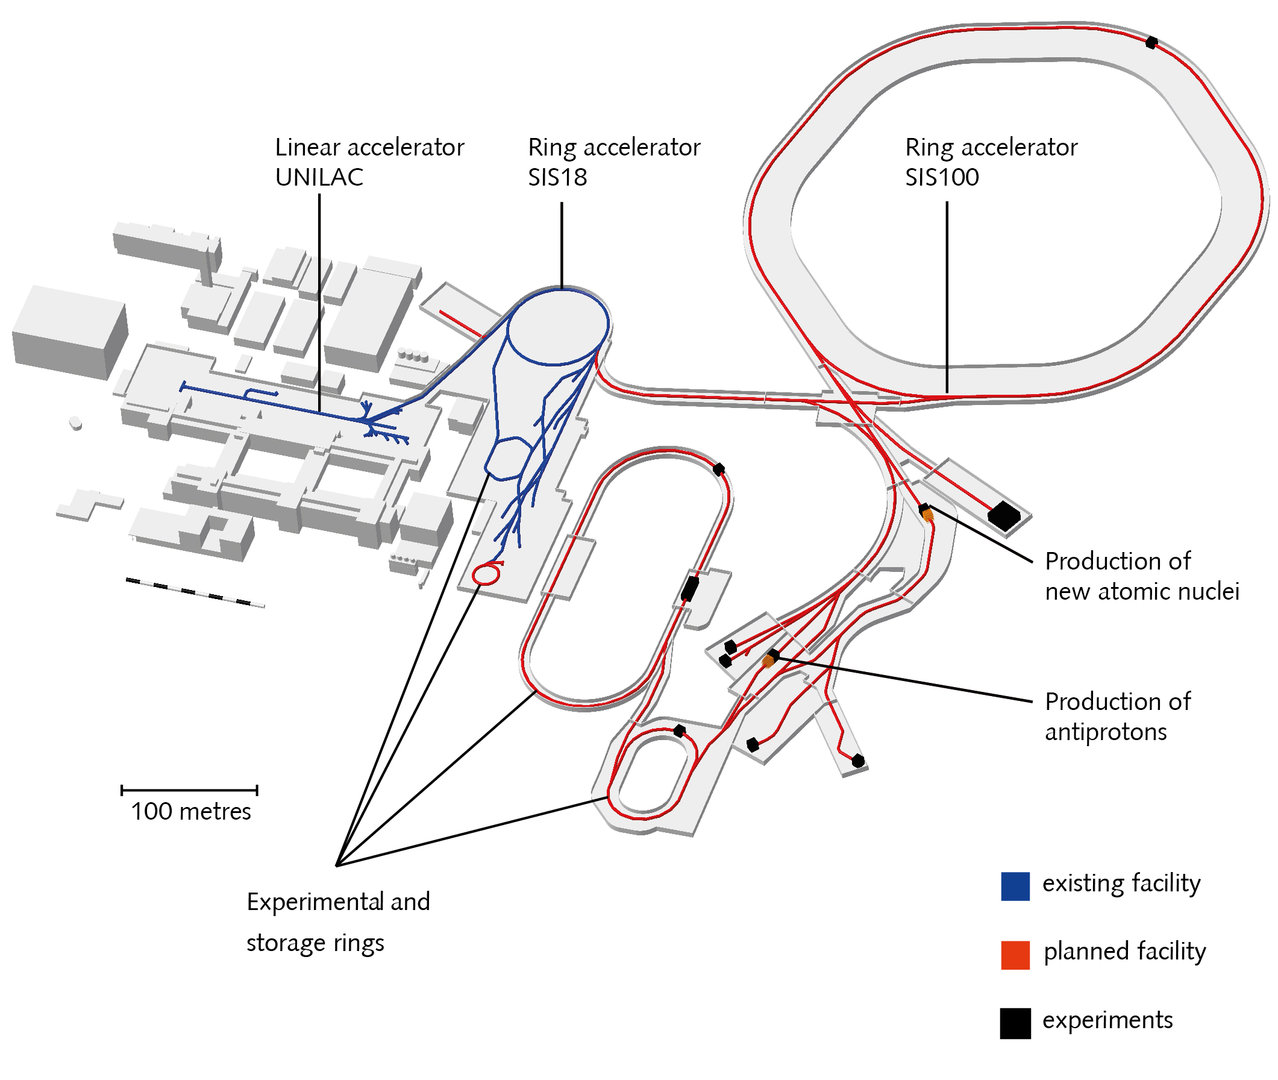
\includegraphics[width=0.65\columnwidth]{Chapter2/images/fair.jpg}
    \caption{Overview of the GSI/FAIR research facility~\cite{fair}}
    \label{fig:fair}
\end{figure}

already existing facility GSI Helmholtzzentrum
für Schwerionenforschung (GSI). Figure 2.2 provides an insight into the infrastructure
currently under construction for FAIR. Facility for Antiproton and Ion
Research in Europe (FAIR) will extend GSI with a more capable accelerator, storage
rings and dedicated experiments from different fields, namely Atomic Physics,
Plasma physics and Applications (APPA), antiProton ANnihilation at DArmstadt
(PANDA), Nuclear Structure, Astrophysics and Reactions (NUSTAR), and Compressed
Baryonic Matter (CBM). The Schwerionensynchrotron 100 (SIS100) is
the accelerator ring built for FAIR and its experiments. The status of SIS100 and
its plans were recently described in Spiller et al

The SIS100 ring accelerator runs along an underground tunnel whose floor lies as deep as 17 meters under the earth’s surface. The SIS100 has a circumference of 1,100 meters and can accelerate the ions of all the natural elements in the periodic table to speeds as high as 99\% of the speed of light. The magnets that keep the ions in their paths are superconducting and are cooled to -269°C by means of liquid helium. The accelerated particles are either used directly for experiments or for the production of other particles, so-called secondary particles
